\documentclass[letterpaper,12pt,fleqn]{article}
\usepackage{matharticle}
\pagestyle{empty}

\newcommand{\e}{\epsilon}
\renewcommand{\d}{\delta}

\begin{document}

\section*{Limit Failures}

\begin{definition}
  To say that \(L\in\R\) is not the limit of a function \(f(x)\) at \(x=a\) means that \(f(x)\not\to L\) as
  \(x\to a\):
  \[\exists\,\e>0,\forall\,\d>0,\exists\,x\in\R,0<\abs{x-a}<\d\ \text{and}\ \abs{f(x)-L}\ge0\]
\end{definition}

Find an \(\e\) such that for every \(\d\), there is at least one \(x\) in the \(\d\)-neighborhood of \(a\) at which
the function value is outside the bounding \(\e-\d\) box.

There are three possibilities:
\begin{enumerate}
\item Gaps
\item Arbitrarily Large
\item Oscillations
\end{enumerate}

\subsection*{Gaps}

\begin{example}[The Heaviside Function]
  Define \(H(x)\) as follows:
  \[H(x)=\begin{cases}
  0, & x<0 \\
  1, & x\ge0
  \end{cases}\]
  Is \(\displaystyle\lim_{x\to0}H(x)=1\)?

  Let \(\e=\frac{1}{2}\).  Note that for any \(\d\), the part of the function for \(x<0\) will always be outside
  the bounding box.

  \bigskip
  
  \begin{center}
    \begin{tikzpicture}
      \draw [->] (-4,0) -- (4,0) node [right] {\(x\)};
      \draw [->] (0,-2) -- (0,4) node [above] {\(H(x)\)};
      \node [open point,blue] (A) at (0,0) {};
      \node [closed point,blue] (B) at (0,2) {};
      \node [left] at (B) {\(1\)};
      \draw [very thick,blue] (-4,0) to (A);
      \draw [very thick,blue] (B) to (4,2);
      \draw [red] (-1,1) rectangle (1,3);
    \end{tikzpicture}
  \end{center}

  \bigskip

  In fact, for any \(L\), an \(\e\) can be selected such that no suitable bounding box can be drawn.

  \begin{center}
    \begin{tikzpicture}
      \draw [->] (-4,0) -- (4,0) node [right] {\(x\)};
      \draw [->] (0,-2) -- (0,4) node [above] {\(H(x)\)};
      \node [open point,blue] (A) at (0,0) {};
      \node [closed point,blue] (B) at (0,2) {};
      \draw [very thick,blue] (-4,0) to (A);
      \draw [very thick,blue] (B) to (4,2);
      \draw [red] (-0.25,2.75) rectangle (0.25,3.25);
      \draw [red] (-0.25,1.75) rectangle (0.25,2.25);
      \draw [red] (-0.25,0.75) rectangle (0.25,1.25);
      \draw [red] (-0.25,-0.25) rectangle (0.25,0.25);
      \draw [red] (-0.25,-1.25) rectangle (0.25,-0.75);
    \end{tikzpicture}
  \end{center}

  \bigskip

  Thus, \(\displaystyle\lim_{x\to0}H(x)\) does not exist (DNE).

  Note that this does not prohibit limits at other values of \(x\).  For example:
  \[\lim_{x\to1}H(x)=1\]
  \begin{center}
    \begin{tikzpicture}
      \fill [lightgray] (1.5,1.5) rectangle (2.5,2.5);
      \draw [->] (-4,0) -- (4,0) node [right] {\(x\)};
      \draw [->] (0,-2) -- (0,4) node [above] {\(H(x)\)};
      \node [open point,blue] (A) at (0,0) {};
      \node [closed point,blue] (B) at (0,2) {};
      \node [left] at (B) {\(1\)};
      \draw [very thick,blue] (-4,0) to (A);
      \draw [very thick,blue] (B) to (4,2);
      \node [closed point,red] (C) at (2,2) {};
      \draw [dashed,red] (C) to (2,0) node [below] {\(1\)};
    \end{tikzpicture}
  \end{center}

  \bigskip

  In fact, for any \(a>0\):
  \[\lim_{x\to a}H(x)=1\]
  and for any \(a<0\):
  \[\lim_{x\to a}H(x)=0\]
\end{example}

\begin{example}
  \begin{minipage}{3in}
    \begin{gather*}
      f(x)=\begin{cases}
      x, & x\le1 \\
      (x-1)^2+2, & x>1
      \end{cases} \\
      \\
      \lim_{x\to1}f(x)\ \text{DNE}
    \end{gather*}
  \end{minipage}
  \begin{minipage}{3in}
    \begin{center}
      \begin{tikzpicture}[scale=0.75]
        \draw [->] (-3,0) -- (3,0) node [right] {\(x\)};
        \draw [->] (0,-3) -- (0,3) node [above] {\(f(x)\)};
        \node [closed point,blue] (A) at (1,1) {};
        \node [open point,blue] (B) at (1,2) {};
        \draw [blue] (-3,-3) to (A);
        \draw [blue] (B) parabola (3,3);
        \draw [dashed] (B) to (A) to (1,0) node [below] {\(1\)};
        \draw [dashed] (B) to (0,2) node [left] {\(2\)};
        \draw [dashed] (A) to (0,1) node [left] {\(1\)};
      \end{tikzpicture}
    \end{center}
  \end{minipage}

  \bigskip

  \begin{minipage}{3in}
    \begin{gather*}
      f(x)=\begin{cases}
      x, & x\le1 \\
      (x-1)^2+1, & x>1
      \end{cases} \\
      \\
      \lim_{x\to1}f(x)=1
    \end{gather*}
  \end{minipage}
  \begin{minipage}{3in}
    \begin{center}
      \begin{tikzpicture}[scale=0.75]
        \draw [->] (-3,0) -- (3,0) node [right] {\(x\)};
        \draw [->] (0,-3) -- (0,3) node [above] {\(f(x)\)};
        \node [closed point,blue] (A) at (1,1) {};
        \draw [blue] (-3,-3) to (A);
        \draw [blue] (A) parabola (3,3);
        \draw [dashed] (A) to (1,0) node [below] {\(1\)};
        \draw [dashed] (A) to (0,1) node [left] {\(1\)};
      \end{tikzpicture}
    \end{center}
  \end{minipage}

  \bigskip

  \begin{minipage}{3in}
    \begin{gather*}
      f(x)=\begin{cases}
      x, & x<1 \\
      2, & x=1 \\
      (x-1)^2+1, & x>1
      \end{cases} \\
      \\
      \lim_{x\to1}f(x)=1
    \end{gather*}
  \end{minipage}
  \begin{minipage}{3in}
    \begin{center}
      \begin{tikzpicture}[scale=0.75]
        \draw [->] (-3,0) -- (3,0) node [right] {\(x\)};
        \draw [->] (0,-3) -- (0,3) node [above] {\(f(x)\)};
        \node [open point,blue] (A) at (1,1) {};
        \node [closed point,blue] (B) at (1,2) {};
        \draw [blue] (-3,-3) to (A);
        \draw [blue] (A) parabola (3,3);
        \draw [dashed] (B) to (A) to (1,0) node [below] {\(1\)};
        \draw [dashed] (B) to (0,2) node [left] {\(2\)};
        \draw [dashed] (A) to (0,1) node [left] {\(1\)};
      \end{tikzpicture}
    \end{center}
  \end{minipage}
\end{example}

\newpage

\subsection*{Arbitrarily Large}

\begin{definition}[Arbitrarily Large]
  To say that \(x\in\R\) is \emph{arbitrarily large}, denoted by \(x\to\infty\) or \(x\to+\infty\), means that:
  \[\forall\,y\in\R,x>y\]
  To say that \(x\in\R\) is \emph{arbitrarily large negative}, denoted by \(x\to-\infty\), means that:
  \[\forall\,y\in\R,x<y\]
\end{definition}

Similar to arbitrarily small, arbitrarily large is an infinite no-win game: given any \(y\in\R\), \(x\) is larger
(greater) than \(y\).

\begin{definition}[Infinite Limit]
  To say that \(\displaystyle\lim_{x\to a}f(x)=\infty\) means that for every \(M>0\), there exists \(\d>0\) such that
  if \(0<\abs{x-a}<\d\) then \(f(x)>M\).

  To say that \(\displaystyle\lim_{x\to a}f(x)=-\infty\) means that for every \(M>0\), there exists \(\d>0\) such that
  if \(0<\abs{x-a}<\d\) then \(f(x)<-M\).
\end{definition}

\begin{example}
  Let \(\displaystyle f(x)=\frac{1}{x^2}\).

  Does \(\displaystyle\lim_{x\to0}f(x)\) exist?

  \bigskip

  \begin{center}
    \begin{tikzpicture}
      \begin{axis}[
          axis lines=middle,
          xmin=-5,
          xmax=5,
          ymin=-1,
          ymax=5,
          ticks=none,
          xlabel={\(x\)},
          ylabel={\(f(x)\)},
          x label style={at={(axis cs:5,0)},anchor=west},
          y label style={at={(axis cs:0,5)},anchor=south},
        ]
        \addplot [domain=-5:-0.25,blue] {1/x^2};
        \addplot [domain=0.25:5,blue] {1/x^2};
        \draw [red] (-0.5,0.5) rectangle (0.5,1.5);
        \draw [red] (-1,2.5) rectangle (1,3.5);
      \end{axis}
    \end{tikzpicture}
  \end{center}

  No matter how the bounding box is drawn, there will be a portion of the function outside of the box since
  \(f(x)\to\infty\) as \(x\to0\).  In fact, for every \(M>0\), a suitable \(\d\) can be found:

  \bigskip

  \begin{center}
    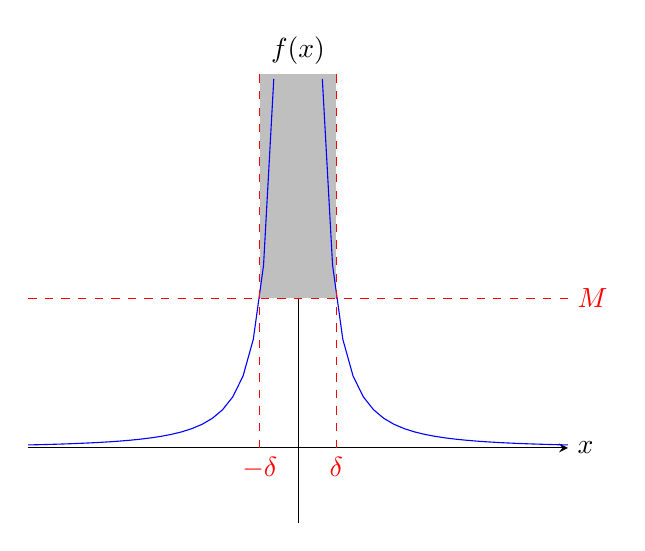
\begin{tikzpicture}
      \begin{axis}[
          axis lines=middle,
          xmin=-5,
          xmax=5,
          ymin=-1,
          ymax=5,
          ticks=none,
          xlabel={\(x\)},
          ylabel={\(f(x)\)},
          x label style={at={(axis cs:5,0)},anchor=west},
          y label style={at={(axis cs:0,5)},anchor=south},
          clip=false
        ]
        \fill [lightgray] ({-1/sqrt(2)},2) rectangle ({1/sqrt(2)},5);
        \addplot [domain=-5:-0.45,blue] {1/x^2};
        \addplot [domain=0.45:5,blue] {1/x^2};
        \draw [dashed,red] (-5,2) -- (5,2) node [right] {\(M\)};
        \draw [dashed,red] ({-1/sqrt(2)},5) -- ({-1/sqrt(2)},0) node [below] {\(-\d\)};
        \draw [dashed,red] ({1/sqrt(2)},5) -- ({1/sqrt(2)},0) node [below] {\(\d\)};
      \end{axis}
    \end{tikzpicture}
  \end{center}

  Likewise: \(\displaystyle\lim_{x\to0}\left(-\frac{1}{x^2}\right)=-\infty\)

  \bigskip

  \begin{center}
    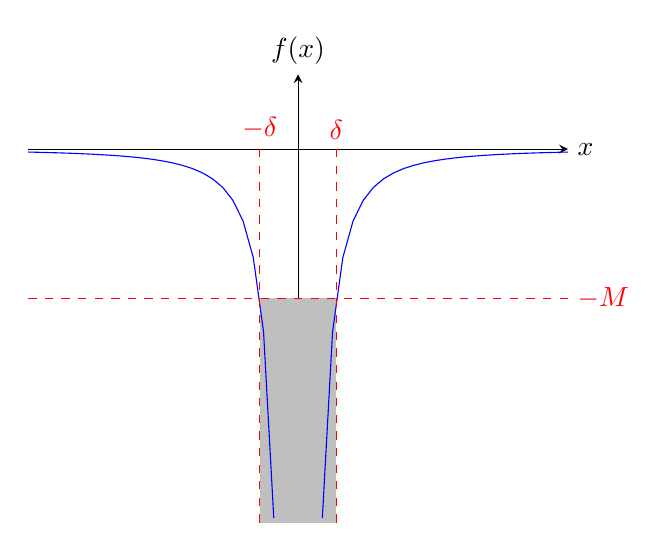
\begin{tikzpicture}
      \begin{axis}[
          axis lines=middle,
          xmin=-5,
          xmax=5,
          ymin=-5,
          ymax=1,
          ticks=none,
          xlabel={\(x\)},
          ylabel={\(f(x)\)},
          x label style={at={(axis cs:5,0)},anchor=west},
          y label style={at={(axis cs:0,1)},anchor=south},
          clip=false
        ]
        \fill [lightgray] ({-1/sqrt(2)},-2) rectangle ({1/sqrt(2)},-5);
        \addplot [domain=-5:-0.45,blue] {-1/x^2};
        \addplot [domain=0.45:5,blue] {-1/x^2};
        \draw [dashed,red] (-5,-2) -- (5,-2) node [right] {\(-M\)};
        \draw [dashed,red] ({-1/sqrt(2)},-5) -- ({-1/sqrt(2)},0) node [above] {\(-\d\)};
        \draw [dashed,red] ({1/sqrt(2)},-5) -- ({1/sqrt(2)},0) node [above] {\(\d\)};
      \end{axis}
    \end{tikzpicture}
  \end{center}
\end{example}

Saying that \(f(x)\to\infty\) or \(f(x)\to-\infty\) as \(x\to a\) is preferred to saying that the limit DNE.

\begin{example}
  Let \(\displaystyle f(x)=\frac{1}{x}\).

  Does \(\displaystyle\lim_{x\to0}f(x)\) exist?

  \bigskip

  \begin{center}
    \begin{tikzpicture}
      \begin{axis}[
          axis lines=middle,
          xmin=-5,
          xmax=5,
          ymin=-5,
          ymax=5,
          ticks=none,
          xlabel={\(x\)},
          ylabel={\(f(x)\)},
          x label style={at={(axis cs:5,0)},anchor=west},
          y label style={at={(axis cs:0,5)},anchor=south},
          clip=false
        ]
        \addplot [domain=-5:-0.2,blue] {1/x};
        \addplot [domain=0.2:5,blue] {1/x};
        \draw [dashed,red] (-5,2) -- (5,2) node [right] {\(M\)};
        \draw [dashed,red] (-5,-2) -- (5,-2) node [right] {\(-M\)};
        \draw [dashed,red] (-1/2,-5) -- (-1/2,5);
        \draw [dashed,red] (1/2,-5) -- (1/2,5);
        \node [below left] at (-1/2,0) {\(-\d\)};
        \node [below right] at (1/2,0) {\(\d\)};
      \end{axis}
    \end{tikzpicture}
  \end{center}

  No matter what the choice of \(M\), part of the graph will always be below (less than) \(M\) and part of the graph
  will be above (greater than) \(-M\).  Thus the limit DNE.
\end{example}

\subsection*{Oscillations}

\begin{example}
  Let \(f(x)=\sin\frac{1}{x}\).

  Does \(\lim_{x\to0}f(x)\) exist?

  \bigskip

  \begin{center}
    \begin{tikzpicture}
      \draw (-5,0) -- (5,0) node [right] {\(x\)};
      \draw (0,-2) -- (0,2) node [above] {\(f(x)\)};
      \draw [domain=-5:-0.01,blue,smooth,samples=1000] plot ({\x},{sin(deg(1/\x))});
      \draw [domain=0.01:5,blue,smooth,samples=1000] plot ({\x},{sin(deg(1/\x))});
      \draw [red] (-0.1,0.4) rectangle (0.1,0.6);
      \draw [red] (-0.1,-0.1) rectangle (0.1,0.1);
      \draw [red] (-0.1,-0.4) rectangle (0.1,-0.6);
    \end{tikzpicture}
  \end{center}

  \bigskip

  For small \(\e\), no matter how small \(d\) is, \(f(x)\) will oscillate outside the bounding box.  Thus, the
  limit DNE.
\end{example}

\begin{example}
  Define \(f(x)\) as follows:
  \[f(x)=\begin{cases}
  1, & x\in\Q \\
  0, & x\in\R-Q
  \end{cases}\]
  Does \(\displaystyle\lim_{x\to2}f(x)\) exist?

  \bigskip

  \begin{center}
    \begin{tikzpicture}
      \draw (-5,0) -- (5,0) node [right] {\(x\)};
      \draw (0,-1) -- (0,2) node [above] {\(f(x)\)};
      \draw [blue!20!white] (-5,1) -- (5,1);
      \draw [very thick,blue] (-5,0) -- (5,0);
      \node [above left] at (0,1) {\(1\)};
      \node [closed point,red] at (2,1) {};
      \draw [dashed,red] (2,2) -- (2,0) node [below] {\(2\)};
      \draw [red] (1.75,0.75) rectangle (2.25,1.25);
    \end{tikzpicture}
  \end{center}
\end{example}

Due to the density of the reals, in any \(\d\)-neighborhood there will be irrational numbers that pull \(f(x)\)
out of the bounding box.  Thus, the limit DNE.

\end{document}
